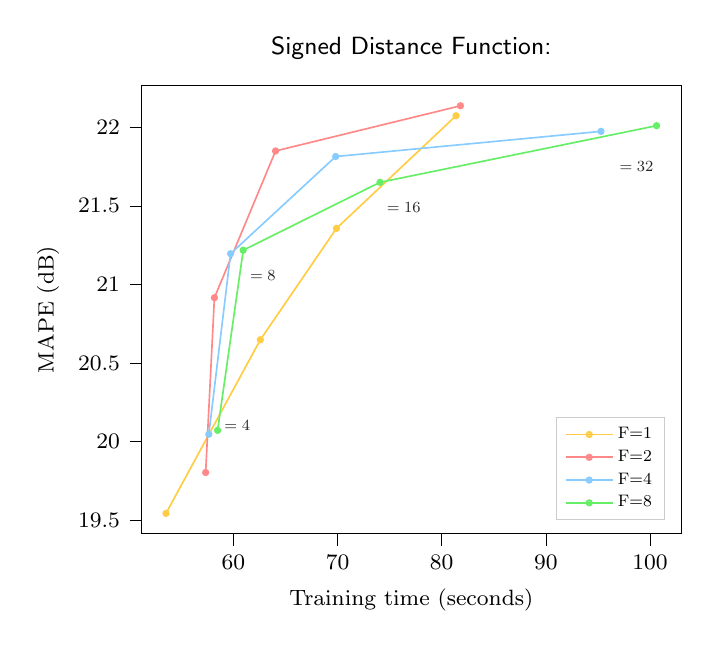
\begin{tikzpicture}
\tikzstyle{every node}=[font=\footnotesize]


\definecolor{color0}{rgb}{1,0.8,0.266666666666667}
\definecolor{color1}{rgb}{1,0.533333333333333,0.533333333333333}
\definecolor{color2}{rgb}{0.533333333333333,0.8,1}
\definecolor{color3}{rgb}{0.4,0.933333333333333,0.4}

\begin{axis}[
legend cell align={left},
legend style={
  fill opacity=0.8,
  draw opacity=1,
  text opacity=1,
  at={(0.97,0.03)},
  anchor=south east,
  draw=white!80!black,
  nodes={scale=0.75, transform shape}
},
tick align=outside,
tick pos=left,
title={{\small \sffamily Signed Distance Function: \sceneCow}},
x grid style={white!69.0196078431373!black},
xlabel={Training time (seconds)},
xmin=51.1697432518005, xmax=102.985850143433,
xtick style={color=black},
y grid style={white!69.0196078431373!black},
ylabel={MAPE (dB)},
ymin=19.4124704903077, ymax=22.266776617726,
ytick style={color=black}
]
\addplot [semithick, color0, mark=*, mark size=1, mark options={solid}]
table {%
53.5250208377838 19.5422116779176
62.5882759094238 20.6477222263526
69.8922746181488 21.3563778278445
81.3737463951111 22.0737044451526
};
\addlegendentry{F=1}
\addplot [semithick, color1, mark=*, mark size=1, mark options={solid}]
table {%
57.3348355293274 19.8022916036004
58.1764385700226 20.9151951390589
64.0480613708496 21.8495327248969
81.8016700744629 22.1370354301161
};
\addlegendentry{F=2}
\addplot [semithick, color2, mark=*, mark size=1, mark options={solid}]
table {%
57.6387646198273 20.0459844079176
59.7291388511658 21.195460470352
69.8229157924652 21.8141258371745
95.2951185703278 21.9742470581402
};
\addlegendentry{F=4}
\addplot [semithick, color3, mark=*, mark size=1, mark options={solid}]
table {%
58.4805581569672 20.0707805516222
60.9406895637512 21.2177000059208
74.0750935077667 21.6497666358274
100.630572557449 22.0103486885545
};
\addlegendentry{F=8}
\draw (axis cs:58.4805581569672,20.0707805516222) node[
  scale=0.7,
  anchor=base west,
  text=white!15!black,
  rotate=0.0
]{$\levels = 4$};
\draw (axis cs:60.9406895637512,21.0237431922275) node[
  scale=0.7,
  anchor=base west,
  text=white!15!black,
  rotate=0.0
]{$\levels = 8$};
\draw (axis cs:74.0750935077667,21.4558098221342) node[
  scale=0.7,
  anchor=base west,
  text=white!15!black,
  rotate=0.0
]{$\levels = 16$};
\draw (axis cs:96.4155711174011,21.7194134680146) node[
  scale=0.7,
  anchor=base west,
  text=white!15!black,
  rotate=0.0
]{$\levels = 32$};
\end{axis}

\end{tikzpicture}
